% 
% Annual Cognitive Science Conference
% Sample LaTeX Paper -- Proceedings Format
% 

% Original : Ashwin Ram (ashwin@cc.gatech.edu)       04/01/1994
% Modified : Johanna Moore (jmoore@cs.pitt.edu)      03/17/1995
% Modified : David Noelle (noelle@ucsd.edu)          03/15/1996
% Modified : Pat Langley (langley@cs.stanford.edu)   01/26/1997
% Latex2e corrections by Ramin Charles Nakisa        01/28/1997 
% Modified : Tina Eliassi-Rad (eliassi@cs.wisc.edu)  01/31/1998
% Modified : Trisha Yannuzzi (trisha@ircs.upenn.edu) 12/28/1999 (in process)
% Modified : Mary Ellen Foster (M.E.Foster@ed.ac.uk) 12/11/2000
% Modified : Ken Forbus                              01/23/2004
% Modified : Eli M. Silk (esilk@pitt.edu)            05/24/2005
% Modified: Niels Taatgen (taatgen@cmu.edu) 10/24/2006

%% Change ``a4paper'' in the following line to ``letterpaper'' if you are
%% producing a letter-format document.

\documentclass[10pt,letterpaper]{article}

\usepackage{cogsci}
\usepackage{pslatex}
\usepackage{apacite}
\usepackage[none]{hyphenat}
\usepackage[compact]{titlesec}

\usepackage[group-separator={,}]{siunitx}

\graphicspath{{./pictures/}} % Specifies the directory where pictures are stored

\title{Predicting Tags for StackOverflow Posts}

\author{{\large \bf Clayton Stanley (clayton.stanley@rice.edu)} \\
  Department of Psychology, 6100 Main Street \\
  Houston, TX 77005 USA 
  \AND {\large \bf Michael D. Byrne (byrne@rice.edu)} \\
  Departments of Psychology and Computer Science, 6100 Main Street \\
  Houston, TX 77005 USA }

\begin{document}

\maketitle

\frenchspacing

\begin{abstract}
  Hashtags created by authors of online content provide a view of a user's goals and interests.
  Predicting users' interests can lead to improved, more user centered human-computer systems.
  Large-scale behavioral datasets such as Twitter, Facebook, LinkedIn, StackOverflow, and Yelp can be mined and explored to study these hashtags and how they relate to users' interests.
  We explored the StackOverflow dataset, and developed an ACT-R inspired Bayesian probabilistic model that can predict the hashtags used by the author of the post.
  The model is 65\% accurate when tasked to predict one tag per post on average.
  This is achieved by choosing the tag that has the highest log odds of being correct,
  given the tag's prior log odds of occurrence and adjusting for the log likelihood ratio of the words in the post being associated with the tag.
  The model is a successful case showing that ACT-R's declarative memory retrieval equations scale, and are relevant to task domains that require large-scale knowledge stores.

  \textbf{Keywords:}
  Tagging; Large-Scale Semantic Memory; Data Mining; ACT-R
\end{abstract}

\section{Introduction}

Human-based tagging of online content has increased in recent years.
A few examples are authors creating hashtags for Twitter tweets and Facebook posts, as well as keywords for research papers.
A large portion of the growing number of social media sites support some sort of human-directed tagging of posts.
Additionally, an increasing number of individuals are using tags as a form of query-based search to find information
(e.g., \citeNP{Diakopoulos2010}).

A growing body of research is focusing on the lifetime and growth characteristics of hashtags for real-time social networking sites such as Twitter
(e.g., \citeNP{Tsur2012, Chang2010}).
However, less is known about the underlying process when choosing particular tags during the creation of the tweet or post.
Modeling tag creation accurately (as opposed to modeling tag growth and behavior after creation) could allow a system to predict the hashtag that a user should use, given the contextual clues available.
There are numerous benefits to this type of tag prediction.
For example, users could be introduced to tags (and potentially communities surrounding those tags) that are of interest to them.
Also tag cleanup systems could be implemented where mistags are identified and corrected.

We built a tag prediction system for the StackOverflow dataset that is intended to solve precisely these sorts of problems.
The StackOverflow dataset was chosen because it is relatively constrained, contains a large number of posts and associated tags, and the data are easy to obtain.
It is constrained because there is a fully enumerated and limited set of tags that an author can use, as opposed to a less-constrained domain such as Twitter.
The site also makes public all post data on a quarterly basis, which can be downloaded and loaded into a database for further analysis.

\subsection{Stack Overflow Dataset}

The StackOverflow dataset consists of all questions and answers posted on stackoverflow.com.
The questions are all related to computer programming and can be posted by anyone with an account, which is free to create.
Each question is tagged by the author with (presumably) the tags that are most representative of the post.
Example tags are programming languages (\emph{PHP}, \emph{Common-Lisp}, \emph{MySQL}, \emph{C\#}) and also general topics (\emph{databases}, \emph{optimization}, \emph{arrays}).
An example post is included in Figure \ref{fig:examplePost}.
Note that the author tagged this post with \emph{javascript}, \emph{firefox}, \emph{dom}, and \emph{svg}.

\begin{figure}[ht]
  \centering
  \resizebox{\linewidth}{!}{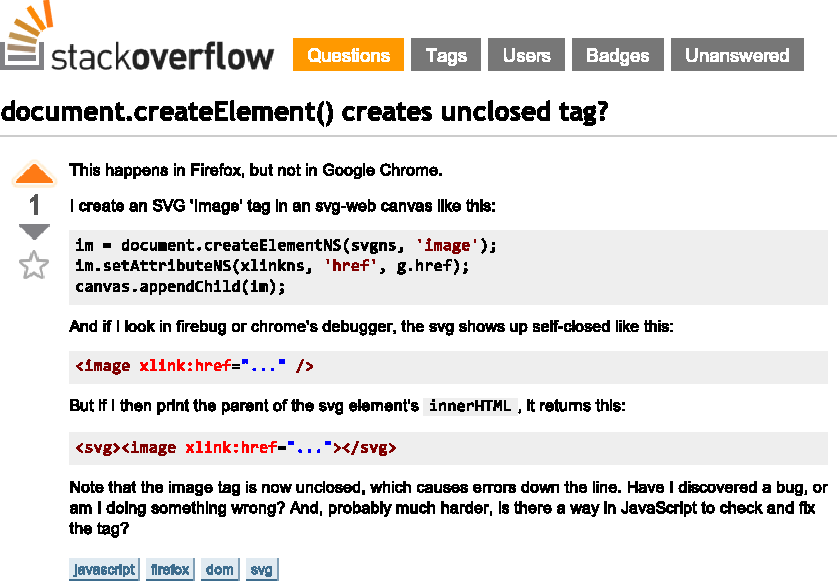
\includegraphics{visPost-2977094-screen-crop.pdf}}
  \caption{Example post on stackoverflow.com}
  \label{fig:examplePost}
\end{figure}

The Apr' 11 dataset \cite{DataDump2011} was used for the analysis.
It contains all posts dated between Jul' 08 (site creation) and Apr' 11.
There are \num{1468485} posts from \num{559803} unique users and \num{26176} unique tags.
Post authors used an average of 2.9 tags per post.

\emph{C\#} is the most often used tag, where about 11\% of posts were tagged with \emph{C\#}.
Tag frequency drops off sharply and approximately follows Zipf's law.
The top 1\% of tags ranked by frequency of use account for approximately 60\% of total tag instances.

\subsection{Related Work}

At least one prior researcher \cite{Kuo2011} has worked on StackOverflow tag prediction.
\citeauthor{Kuo2011} uses a co-occurrence model that predicts tags based on the words in the post and their relation (co-occurrence) to tags.
The model was initially built for next-word prediction in large documents, and then adapted to the StackOverflow dataset by constraining the next word predicted to only tags.
His co-occurrence model has a 47\% classification accuracy predicting one tag per post.

The SNIF-ACT \cite{Fu2007} model also uses co-occurrences and can predict link traversal for search queries.
That is, given a search query (goal state) and fetched results, the model predicts the most likely link that a person will click on.
This StackOverflow model is similar because it leverages ACT-R's declarative memory retrieval mechanisms to generate predictions (tag activations instead of link activations).
However, it is slightly different because it takes into account prior odds of tag activations which was not necessary in SNIF-ACT.

\section{Model}

The tag prediction model is a cognitively-inspired Bayesian probabilistic model based on ACT-R's declarative memory retrieval mechanisms \cite{Anderson2004}.
These equations describe the likelihood that a chunk from memory will be retrieved, given the prior odds of retrieving the chunk and the current context.
So the task of retrieving the tag with the highest activation from the words in the post is similar to performing a declarative memory retrieval request for a tag, given the context of title and body words.
The hypothesis is that the tags used for posts are based on a tag's history of prior use and the strength of association between the tag and the content of words in the title and body of the post.

\vspace{-1em}

\renewcommand{\arraystretch}{1.5}
\renewcommand{\tabcolsep}{.5mm}
\begin{table}[!ht]
  \begin{center}
    \caption{The StackOverflow tag prediction model}
    \label{sample-table}
    \vskip 0.12in
    \begin{tabular}{ll}
      \hline
      Common Name &  Equation \\
      \hline
      Activation & 		$A_{i} = B_{i} + \sum_{j\in T}^{ } W_{j} S_{ji} + \sum_{j\in B}^{ } W_{j} S_{ji} - O$ \\
      Base Level & 		$B_{i} = log \frac{p_{i}}{1-p_{i}}$ \\
      Strength Assoc. &		$S_{ji} = log \frac{p(i|j)}{p(i))} = log \frac{NN_{ji}}{N_{Row}(j)N_{Col}(i)}$ \\
      Co-occurrence &		$N_{ji} = \sum_{}^{}{observed_{ji}}$ \\
      Observations &		$N = \sum_{}^{}{\sum_{}^{}{N_{ji}}}$ \\
      Attention Weight	& 	$W_{j} = W \frac{E_{j}} {\sum_{}^{} {E_{j}}} $ \\
      Scaled Entropy & 		$E_{j} = 1-\frac{H_{j}}{H_{max}}$ \\
      Entropy & 		$H_{j} = -\sum_{i=1}^{N}p(i|j)log\left (  p(i|j) \right )$ \\
      Offset & 			$O = \frac{1}{5}\sum_{i\in top 5}^{ } A_{i}$ \\
      \hline
    \end{tabular}
  \end{center}
\end{table}

Table \ref{sample-table} includes a formal description of the model.
Here, the $i$ subscript denotes activation for a particular tag $i$, and the $j$ subscript is for context.
$A_{i}$ is total activation for tag $i$.

Similar to SNIF-ACT \cite{Fu2007}, we interpret ACT-R's activation equation as a Bayesian prediction of the likelihood of retrieving a tag, given the tag's prior and updated by context.
That is, the log odds of retrieving a particular chunk or tag ($A_{i}$) is determined by adjusting the tag's prior log odds ($B_{i}$) with new information ($\sum_{}^{} W_{j} S_{ji}$).
The main difference is that an offset term ($O$) was included for the StackOverflow model, which is not present in SNIF-ACT or ACT-R's retrieval equations.

\subsubsection{Base-Level Activation}

Base-level activation ($B_{i}$) is the prior log odds of an author using tag $i$.
The prior log odds are based on both frequency and recency of use.
However, we are assuming that frequency of tag use does not change greatly between Jul' 08 and Apr' 11 (time period of dataset).
This is a reasonable assumption for the StackOverflow dataset, since tags relate to programming languages, and the rank of programming-language popularity has not changed drastically within the past few years.
This also makes calculating the priors computationally tractable for this large-scale dataset, because the prior log odds can be computed based on frequency only, as is indicated in Table \ref{sample-table}.
So the tag with the highest frequency (\emph{C\#}) would have the highest base-level activation.

\subsubsection{Contextual Activation}

Contextual activation can be thought of as the amount of odds adjustment to base levels, given the current context $j$.
Contextual activation has two components: strength of association ($S_{ji}$) and attentional weight ($W_{j}$).
Strength of association measures the relatedness of a contextual element $j$ (e.g., the word PHP in the title of a post) with a tag $i$ (e.g., the tag \emph{PHP5}).

\subsubsection{Attentional Weighting}

Attentional weighting ($W_{j}$) can be thought of as the amount of attentional resources that are dedicated to contextual element $j$.
Total attentional weighting ($W$) is bound, most often set to 1, and reflects the fact that attentional resources are limited.
For the StackOverflow model, the attentional weighting was left unbound and allowed to be calibrated by the logistic regression model.
This was done for two reasons:
First, the we were curious to see what value the logistic regression model would give for $W$.
Second, a non-ACT-R standard measure of attentional weighting was used ($E_{j}$), so it seemed appropriate to allow $W$ to vary alongside exploring this new weighting measure.

\subsubsection{Entropy}

During initial model testing, the attentional weighting for all words was equal and set to $W/n$ for $n$ title words (set similarly for body words).
The problem with this approach is that words like ``the'' and ``?'' that are often observed across all tags (i.e., ``stop words'') have the same attentional weighting as highly predictive words like ``PHP''.
Granted the $S_{ji}$'s across all tags for stop words like ``the'' are much lower (and more evenly distributed) than the few $S_{ji}$'s that spike for ``PHP'' (e.g., the tag \emph{PHP}).
However, this still seemed problematic for two reasons:
First, one could argue that stop words are simply adding error in the model's tag activation calculation because they are observed evenly across all tags.
Second, because $W$ is held constant across posts, any attentional resources that are allocated to stop words are unavailable for highly predictive words.

It is also the case that there are many commonalities between ACT-R's declarative memory retrieval equations and other non-ACT-R information retrieval theories,
and many of those theories use a combination of weighting schemes for contextual relevance and global importance of a particular chunk.
For example, \citeA{Dumais1991} shows that a measure of how likely term $j$ is in document $i$ is often the product of a local weighting $L_{ji}$ and global weighting $G_{j}$ measure.
This idea maps cleanly to ACT-R's equations: 
Terms are context words $j$, documents are tags $i$, local weighting is strength of association $S_{ji}$, and global weighting is attentional weight $W_{j}$.

So the scaled entropy measure $E_{j}$ was chosen as a global weighting measure for this dataset because it has a strong theoretical foundation and it predicts well \cite{Dumais1991}.
It is based on Shannon's Information Theory, which measures the amount of information content (predictiveness) of a word.
So the scaled entropy ($E_{j}$) of a context word can be thought of as the amount of predictiveness that that word has to \emph{any} tag.
This means that a stop word like ``the'' will have a scaled entropy measure close to 0, while a highly-predictive word like \emph{macro} will have a scaled entropy measure close to 1.
Looking at $W_{j}$, if $E_{j}$ is low then $W_{j}$ is low, meaning that the scaled entropy measure helps allocate limited attentional resources to predictive contextual elements.

\subsubsection{Offset}

An offset measurement (mean of the top five tags for the post) was used to equalize the top activated tags across posts.
This was done primarily to improve model fit.
To see why this is the case, consider the following scenario:
The offset measurement is not used, and the model is asked to provide ten tags across ten posts.
The top ten tags for one of these posts have activations that are higher than activations for all other tags in the other nine posts.
The model would then select the ten tags from the single post as the most likely tags.
But this does not make sense, because there is a limit to the number of tags that people tend to use for each post.
So the offset measure aims to place all of these ten posts on the same level, so that asking the model to choose ten tags from ten posts will select roughly a single tag from each post.

\section{Method}

\subsubsection{Summary}

A variation of ACT-R's declarative memory retrieval theory \cite{Anderson2004} was used to model tag retrievals for StackOverflow posts.
The strength of association between post words and tags was calculated using 2/3 of the dataset (one million posts).
A logistic regression statistical technique was used to calibrate model parameters and optimize performance.
The weights for each model component were calibrated using a sample of \num{1000} posts not contained within the strength of association dataset.
The calibrated model was then tested on a fresh sample of \num{1000} posts.
Classification accuracy was used as a metric of model performance (i.e., number of correctly-predicted tags).

\subsection{Generating Model Predictions}

For a given title and body of a post, the model returns the activations for each possible tag.
The tag with the highest activation is the most likely tag to be associated with that post.

The R statistical programming environment was used to build the model and generate model predictions.
One million posts (approximately 2/3 of all posts) were loaded into R to build the co-occurrences and tag occurrences.
In order to generate a model prediction, tag activations for title and body context were computed separately, and then added to each tag's prior base-level activation.
An offset constant (equal to the average activation of the top 5 model-predicted tags for the post) was then subtracted from the prior value.
The resulting tags were rank sorted, and the one with the highest activation is the model's prediction of the most likely tag associated with that post.

\subsubsection{Measuring Co-occurrences}

Model tag predictions are based on the amount of word co-occurrences between words in the post and tags used for that post.
To build the co-occurrence matrix between post words and tags, all title and body text and associated tags were extracted from the relational database.
The Python Natural Language Processing Toolkit \cite{Bird2009} was used to chunk (i.e., tokenize and lemmatize) the text in the post.
The tags were already chunked, but tag synonyms were converted to their root tag using the community-maintained StackOverflow tag synonym database.
Afterwords the processed word chunks and root tags were imported into a PostgreSQL table.

A query was then used to build the post word, tag word co-occurrence matrix.
There are \num{39223968} unique post word, tag word combinations.
The result was a table of co-occurrence counts for each of the combinations, which was loaded into R.

\subsubsection{Measuring Tag Occurrences}

Model tag predictions are also based on the frequency that each tag has been used.
More often used tags have a higher base-level activation.
A SQL query was used to build a similar table of tag use counts for the \num{26176} unique tags, which was loaded into R.

\subsubsection{Entropy and Stop Words}

\citeA{Bird2009} recommended the removal of low-predictor stop words from the analysis.
\citeauthor{Bird2009} provided a short list that were commonly removed (e.g., ``the'', ``and'', ``or'').
However it seemed somewhat arbitrary to remove an explicitly-enumerated list of stop words.
Looking at the scaled entropy measure, it seems quite plausible that this measure of word predictiveness can also be used to identify stop words.
That is, words with scaled entropy close to zero \emph{are} the stop words.
Looking at the lowest ten scaled-entropy words for this dataset, (``does'', ``anyone'', ``'ve'', ``found'', ``are'', ``seems'', ``has'', ``been'', ``for'', ``support''),
using scaled entropy to determine stop words works fairly well.
So instead of explicitly removing an enumerated list of stop words, we used a data-driven approach and let the scaled entropy measure attenuate the words that were not predictive of any tag to near-zero levels.

\subsection{Measuring Model Fit}

For a given post, the model produces a vector of tag activations.
For that post, the author's chosen tags are known (see Figure \ref{fig:examplePost}).
So model performance can be measured by comparing the model's tag activations with chosen tags for a post, and then aggregated across posts to get an average.

A logistic regression technique was used to operationalize this fit measure.
For each post, three sets of tag groups were combined to most accurately sample tag activations while managing computer resource constraints:
The top 20 tags having the highest model activation, a random sample of 400 tags, and the tags that were chosen by the author of the post.
Each of these observations was assigned a category of 0 or 1 depending on if the tag was a chosen tag or not for that post (0 is not chosen).
Conceptually, if the model has good categorization power, the observations assigned 1 should have higher tag activations than the observations assigned 0.

These vectors of tag activation, categorization were collected across a set of \num{1000} fresh posts that were not used to train the model on word association strength.
The parameters were optimized to best predict categorization (chosen tag, not chosen tag) from the four predictor variables:
The tag's prior occurrence frequency, word co-occurrence activation for title and body words, and activation offset for the post.

However using a single run of the \num{1000} posts was insufficient because there are two model components that require prior estimates of coefficients:
The offset measure to determine the top-five tags and associated activation and the sampling technique used to pick the top 20 model-predicted tags for each post.
So model calibration was bootstrapped, where the coefficients from the previous run were used as estimates of coefficients for the next run.
The coefficients converged on best-fit values quickly (only required two sets of four iterations), and did not show any signs of instability.

\section{Results}

\subsubsection{Logistic Regression}

\vspace{-1em}

\renewcommand{\arraystretch}{1}
\renewcommand{\tabcolsep}{1mm}
\begin{table}[!ht]
  \begin{center}
    \caption{Best-fit coefficient estimates from logistic regression}
    \label{tab:coeffs}
    \vskip 0.12in
    \begin{tabular}{lllll}
      \hline
      Coefficient & 	Estimate &	Std. Err. &	z value &	$Pr(>|z|)$  \\
      \hline
      (Intercept) &	-2.22 &		0.10 &		-22.95 &	\textless2e-16 *** \\
      prior &		0.62 & 		0.01 &		66.94 & 	\textless2e-16 *** \\
      Wtitle &		0.93 &		0.02 &		40.00 &		\textless2e-16 *** \\
      Wbody &		1.75 &		0.04 &		43.16 &		\textless2e-16 *** \\
      offset &		0.78 &		0.02 &		33.25 &		\textless2e-16 *** \\
      \hline
    \end{tabular}
  \end{center}
\end{table}

\renewcommand{\arraystretch}{1}
\renewcommand{\tabcolsep}{3mm}
\begin{table}[!ht]
  \begin{center}
    \caption{Model fit metrics}
    \label{tab:fits}
    \vskip 0.12in
    \begin{tabular}{ll}
      \hline
      Common Name &  Value	\\
      \hline
      McFadden's Pseudo $R_{}^{2}$ &	.52 \\
      True Positives &			507 \\
      False Positives &			216 \\
      True Negatives &			\num{417408} \\
      False Negatives &			\num{2375} \\
      Positive Predictive Value &	0.70 \\
      Negative Predictive Value &	0.994 \\
      \hline
    \end{tabular}
  \end{center}
\end{table}

The final best-fit coefficients for each model component and statistical measurements are included in Tables \ref{tab:coeffs} and \ref{tab:fits}.
All four coefficients for the run are strong predictors of tag use ($p<.01$), and model fit is satisfactory (McFadden's pseudo $R_{}^{2}=.52$, npv = .994, ppv = .70).
It is also interesting that although the attentional weighting ($W$) terms for the title and body were calibrated by the regression, they did not stray far from cognitively-plausible defaults
(see coefficients for title and body in Table \ref{tab:coeffs}).

\subsubsection{Example Posts}

A visualization of the model's tag activation for the post in Figure \ref{fig:examplePost} is included in Figure \ref{fig:modelPost}.

\begin{figure}[ht]
  \centering
  \resizebox{\linewidth}{!}{\includegraphics{visPost-2977094-act-crop.pdf}}
  \caption{
    Model's prediction of the top tags for post in Figure \ref{fig:examplePost}.
    At the top is the title text of the post, then the attentional weight (scaled entropy) for each word in the title, then the user-chosen tags.
    The bar graphs are the total activation for the top predicted model tags for the post.
    Each bar graph is partitioned into the three model components that vary across the tags in a single post.
}
  \label{fig:modelPost}
\end{figure}

The base level activation and contextual activation combine to predict tags that are both frequently used and contextually relevant.
For example, note that the \emph{javascript} tag leverages a combination of contextual activation and prior activation to achieve a high total activation.
Alternatively, the \emph{svg} tag relies almost entirely on context to achieve high activation.
And note that the model is by no means perfect.
For example, \emph{html} and \emph{jquery} are not tagged by the author, but the model ranks them as the second and third highest tag.
And the author's tag \emph{firefox} is only ranked 12th by the model.

\subsubsection{Generalizability}

In order to test how well the model (and calibrated parameters) generalize to the rest of the StackOverflow dataset,
model parameters were held constant and the model was tested on a fresh set of \num{1000} posts.
Model classification accuracy as a function of number of tags predicted by the model was used as the metric to test if the model generalized.

\subsubsection{Classification Accuracy}

A plot of model performance for both the calibration and test runs is included in Figure \ref{fig:ROC}.

\begin{figure}[ht]
  \centering
  \resizebox{\linewidth}{!}{\includegraphics{ROC-crop.pdf}}
  \caption{
    Model performance across the calibration and test dataset, as well as when specific model components are removed.
    The y-axis is model performance (one is perfect), and the x-axis is the proportion of tags that the model generates compared to the total number of tags used by the post authors (one is equal number).
    The vertical dotted line is where the model generates one tag per post on average.
  }
  \label{fig:ROC}
\end{figure}

Note how model performance is almost identical for the calibration and test dataset (compare full model calibration to full model test), which indicates that model parameters generalize well.
There is a small decrease in performance for test compared to calibration to the left of the vertical dotted line, and model performance at the dotted line is slightly lower (65\% compared to 67\%).
Model performance for the test dataset (cross-validated performance) is the most accurate measurement of real-world performance,
and model accuracy is 65\% for this dataset when tasked to predict one tag per post on average.

\subsubsection{Necessity Analysis}

Figure \ref{fig:ROC} also shows performance after specific model components are removed.
Model parameters were recalibrated for each model, except for the full model test dataset that used the parameters from the calibration dataset.
These plots provide useful information regarding the relative necessity of each component in the full model.
That is, which model components contribute most strongly to increased performance, and which model components might be redundant (not necessary).
Note that it is certainly the case that each model component contributes positive and unique variance to model performance.
However, removing only one component (particularly the words in the body of the post) does not drastically reduce model performance.
It is only when groups of components are removed that model performance starts to drastically suffer.

\section{Discussion}

Our StackOverflow model is a successful case showing that ACT-R's declarative memory retrieval mechanisms scale, and can be applied to retrieval requests occurring across large-scale declarative memory datasets. 
The model can successfully tag 65\% of posts correctly, when tasked to predict one tag per post on average.
The model is also computationally space efficient:
Large-scale relational database techniques and efficient sparse matrix data structures were used for implementation,
so that the data structures require only 3GB of memory and retrieval requests with a DM dataset of \num{556677795} chunks occur in less than one second on a single processor.
Although certainly not perfect, model accuracy is significant and retrieval times are fast, so we are considering potential applications of the model in real-world settings.

\subsubsection{Potential Applications}

The model could be deployed as a tag recommender system for stackoverflow.com. 
If a post author does not include the model's predicted best tag for the post, then the model could suggest the tag to the author.
This would provide a way to introduce authors to tags that are contextually relevant to their interests that they may not have been aware of.
This could also improve the answers received for the post, since other expert programmers may have only been monitoring the model's predicted best tag for the post.

The model could also be used as a tag cleanup system.
In this scenario the tags for a previously submitted post would be compared against model predictions.
If the model's predicted tag activation for a used tag is substantially low, then that tag could either be removed from the post, or the post could be flagged for further analysis.

\subsubsection{Comparison to \citeA{Kuo2011}}

Our model achieves 65\% classification accuracy when predicting one tag per post on average (see Figure \ref{fig:ROC})
compared to 47\% accuracy for the co-occurrence model presented in \citeA{Kuo2011}.
Most likely we achieved the increase in model performance by adding the offset model component and possibly the body term as well, 
as it was unclear if \citeauthor{Kuo2011} used context from both the body and title of a post or just the title.
Also we used two orders of magnitude more posts to train the model co-occurrence matrix ($S_{ji}$).
Nonetheless, there are certainly model similarities:
Co-occurrence count was used as the core measure of similarity, and both local (strength of association) and global (entropy or idf) weighting measures were used to compute tag likelihood, given context.

\subsubsection{Entropy and ACT-R's Attentional Weighting}

Model performance improved by using a scaled entropy measure to weight the importance of each contextual element in the body and title of a post.
However, it is uncommon for an ACT-R model that uses the declarative memory retrieval mechanisms to use anything other than equal attentional weighting for each chunk in context.
But it is much more common outside of the ACT-R modeling community to use both a local (strength of association) and global (attentional weight) term to predict document retrieval \cite{Dumais1991}.
In fact, it has been shown that the Pointwise Mutual Information Index (PMI) (a commonly-used measure to predict document retrieval)
is mathematically equivalent to ACT-R's retrieval equations when the sample size of the corpus is large \cite{Budiu2007, Farahat2004},
and both global and local weightings are commonly used when the PMI measurement is used.
This suggests that using a global weighting term for chunks in context (e.g., the scaled entropy measure used here)
alongside the more commonly-used local weighting (spreading activation) might be useful for other ACT-R models that are taking advantage of large declarative memory datasets to build up the model's base knowledge.

\subsubsection{Model Plausibility}

ACT-R's declarative memory retrieval process makes up the core of the StackOverflow model.
This is a more constrained and cognitively-plausible model than the set of general machine learning techniques used by \citeA{Kuo2011} for the same task. 
Interestingly, when using ACT-R's retrieval mechanism, the model performs significantly better than the less constrained models in \citeA{Kuo2011}.
So there is no reason to think that people do not engage in a process much like this to select tags.
However, more research is necessary before making the strong claim that the StackOverflow model \emph{is} the process people go through when selecting tags on the site, or tags in general.
In particular, the tag errors made by authors should be analyzed, and model behavior should be tested against these important counter examples.
Also, places where the StackOverflow model deviates from ACT-R's default retrieval theory (i.e., the offset term, entropy and attentional weighting) should be examined in greater detail.

\subsubsection{Current Model Issues}

Including the offset term in the model improved performance (see Figure \ref{fig:ROC}).
However by normalizing the top activations for all posts, the model cannot differentiate between a post where the top predicted tag is certain, and a post where the top-predicted tag is questionable.
One could argue that normalizing top activations for all posts should cause model performance to decrease, and the opposite was actually observed.
One hypothesis is that this normalization is required because the retrieval threshold of a tag is adjusted for each post, and changed so that only a small set of tags are retrieved for all posts.
Further research will explore this and other theories for the behavior of the offset component.

\subsubsection{Future Planned Research}

Alongside exploring the offset component and cognitive plausibility, our main planned research is to include the post author's past tagging behavior as an additional model predictor.
We are exploring a Bayesian updating technique that would adjust prior tag activations from global priors to user's priors as more tagging information about the user is collected.
For the StackOverflow dataset, adding user's tagging history to the model should improve predictive power for veteran users,
since programmers tend to specialize on a few set of tags that are of interest to them.

\section{Acknowledgments}

We would like to thank Fred Oswald for his excellent guidance and feedback throughout the model development process.

\bibliographystyle{apacite}
\setlength{\bibleftmargin}{.125in}
\setlength{\bibindent}{-\bibleftmargin}
\bibliography{bibliography}

\end{document}
